\section{Proposed Approach}\label{sec:approach}
A high-level description of the skip list has been already introduced in the previous section. This section provides implementation details about the proposed lock-free skip list using C++11 and its atomic operations.\\
Like most lock-free data structures, we had to deal with the problem that a predecessor node can be deleted by another concurrent operation which would lead into incorrect behavior. This is known as the {\em predecessor-deletion} problem, and it is graphically described in figure XX.\\%[FIND BETTER WORD, see paper]. 
A common approach is adding a delete flag to each node and performing a lazy deletion. However, this implies doing an imperative Compare-and-Swap (CAS) operation on the {\em next} pointer and the delete flag simultaneously. Multiple implementation alternatives are possible: {\em Atomic Markable Reference}, double CAS, double-width CAS, Transactional-Memory. For our data structure we implemented an {\em Atomic Markable Reference} type by using the least significant bit as a deletion flag. Thereby we are able to use the C++11 {\em compare\_and\_exchange} operation.
There are not expected issues when using the least significant bit as a deletion flag as long as the deletion flag is marked out before dereferencing the pointer.\\
In addition to the common skip list methods (e.g. empty, size, find, remove, insert), we added a \textit{pop} method, which is required for a priority queue, and also batch processing methods for inserting or removing \textit{k} elements. The interface of our implementation is shown in [].\\


\begin{lstlisting}[language=C++,basicstyle=\tt\footnotesize,captionpos=b,caption=PPQ interface,morekeywords={*, size_t}]
template <class T, class Comp> class PPQ
{
	bool empty() const;
	size_t size() const;
	bool push(const T& data);
	size_t push(T data[], int k);
	bool remove(const T& data);
	bool pop_front(T& data);
	size_t pop_front(T data[], int k);
	bool contains(T data);
	void print();
};
\end{lstlisting}

\subsection{Correctness verification}
\label{subsec:corr_ver}
We used two different applications for verifying the correctness of our algorithm, a lossless data compression algorithm and an algorithm to find the shortest path in a graph. 
%\mypar{Huffman coding algorithm}
As a first correctness test for single threaded execution a Huffman encoding algorithm was implemented which makes use a priority queue. The algorithm can either use an existing Min-heap implementation or our own skip list based implementation. For a variety of inputs the outputs the two variations were compared to verify correctness.
%We implemented the Huffman coding algorithm as an initial correcteness test for our data structure implementation. This algorithm consists in two main steps. The first step is to initialize a data structure which keeps all the items sorted by their frequency. Then in a second step, it iterates until the data structure has a single element. Every iteration consists of picking the two nodes with the lowest frequency/probability, creating a parent node out of them with the sum of the children's frequencies/probabilities, inserting this new node into the data structure and assigning code zero, or one to the children, and delete them from the data structure. We compared the output of a Huffman coding algorithm using a min-heap with an implementation using our priority queue. We only compared correctness between this two implementations as this loseless compression algorithm is based on iterating linearly through the elements of the underlying data structure and no concurrent access is done.
%\mypar{Shortest path algorithm}
A second correctness test was based on a shortest path algorithm which is part of Intel's TBB source code. In it original version it makes use of the \textit{concurrent\_priority\_queue} of TBB, we adapted the algorithm such that it can also use our own lock-free implementation instead. In contrast to the previous test, this algorithm accesses the priority queue concurrently. Like before the outputs of the two variations for different input graphs were compared to verify correctness. Performance measurement for these algorithms were not conducted since it might have implied tuning the algorithms itself and not just the priority queue. Which would not be in the scope of this project. In section~\ref{sec:exp} performance evaluation against TBB's \textit{concurrent\_priority\_queue} is presented for specific workloads.

\subsection{Memory allocation micro-benchmark}
Early measurements indicated that memory allocation on the Xeon Phi might represent a significant part of the runtime. Therefore we performed a micro-benchmark to benchmark the memory allocation process on the Xeon Phi. Three different allocators were considered. The default c++ allocator, the default TBB allocator and the TBB scalable allocator. 

Intel TBB scalable allocator uses \textit{thread-private heaps} to reduce the amount of code that needs synchronization and avoids false sharing. Each thread allocates its own copy of heap structures and accesses it via thread-specific data (TSD) using corresponding system APIs.
The allocator gets 1\,MB chunks from the operating system and divides them into 16\,Kbyte aligned blocks. Then, it places these blocks initially in a global heap of free blocks. Memory request from the application can be served from this heap, if the heap holds no more free blocks. The allocator will again request a big chunk of memory from the operating system. Further the heap of free blocks memory re-usage by adding freed memory to the heap instead of returning it directly to the operating system. Additional blocks are requested if a thread does not find free objects in the blocks of its own heap and there are no available blocks in the global heap~\cite{_thefoundations,Hudson:2006:MST:1133956.1133967}. %In order to use the scalable allocator offered by Intel TBB, the TBB and its allocator library were linked to our benchmarks.

\begin{lstlisting}[language=C++,basicstyle=\tt\scriptsize,captionpos=b,caption=Lock free node structure,label=lst:freenode,morekeywords={*, size_t}]
template <typename T>  struct LockFreeNode
{	
	T data;
	int	level;
	AtomicRef<LockFreeNode>	next[0];
};
\end{lstlisting}

Furthermore, we performed dynamic allocation of the {\em next} pointer array in order to ensure that each skip list node can be cache-aligned. Listings~\ref{lst:freenode} and~\ref{lst:fn_alloc} show code snippets of how this was accomplished.
\begin{lstlisting}[language=C++,basicstyle=\tt\scriptsize,captionpos=b,caption=Memory allocation instruction for array of atomic references,label=lst:fn_alloc, morekeywords={*, size_t}]

scalable_malloc(
sizeof(LockFreeNode) 
+ 
((arrayLength + 1) * sizeof(AtomicRef<LockFreeNode>))
)
\end{lstlisting}

We designed our micro-benchmark to allocate ten million skip list nodes while using 240 threads. We measured the time it takes to allocate that many elements on the Xeon Phi. As expected the C++ default allocator has a much higher runtime than the two TBB allocators. In numbers these two allocators obtained a 24 respectively 38 times improvement over the C++ default allocator. The results are displayed in figure~\ref{fig:mem_alloc}.

\begin{figure}
	\centering
  	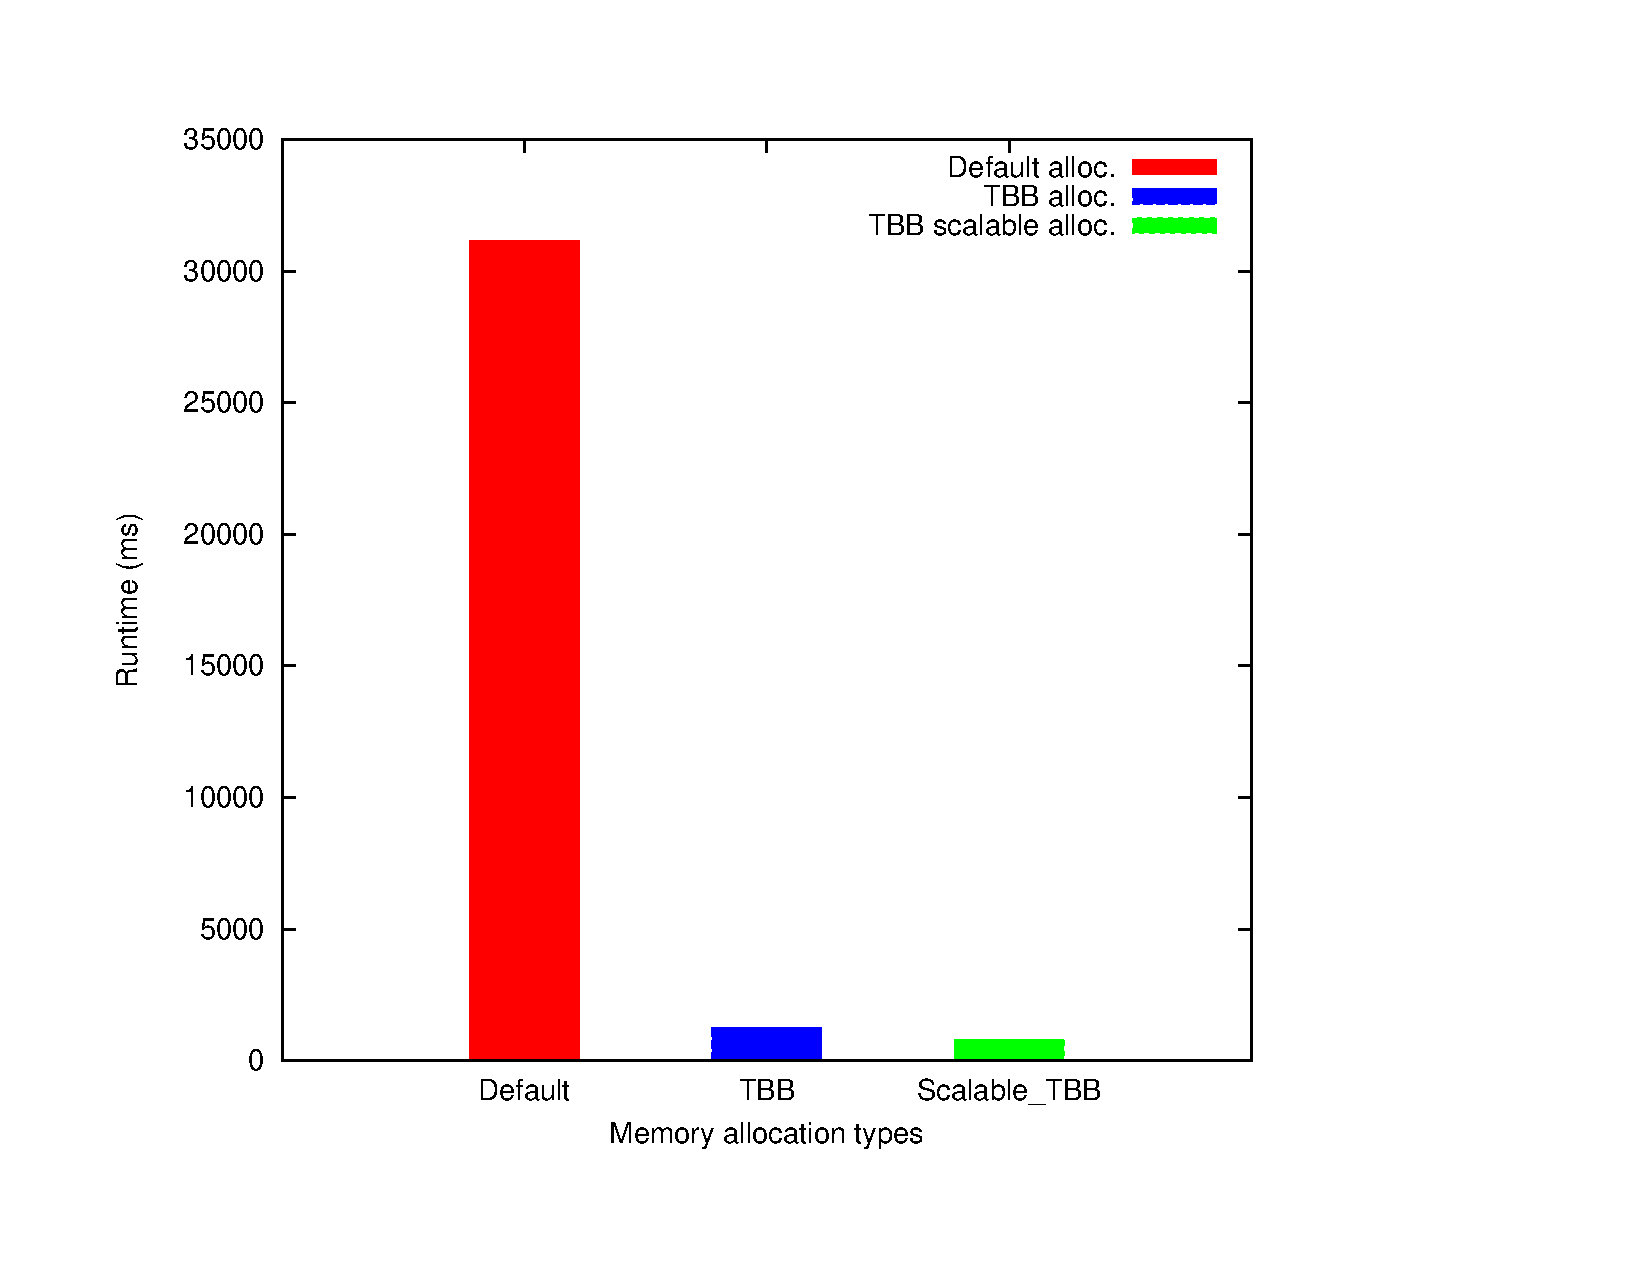
\includegraphics[scale=0.3]{../plots/mem_alloc/mem_alloc.pdf}
	\caption{Memory allocation runtime for C++ default, TBB default and TBB scalable allocator.}
	\label{fig:mem_alloc}
\end{figure}
